\section{Linearization of the Perturbed Equations of Motion in Position and Velocity Space}

Since perturbations are supposed to be ``small effects'' one approach to linearizing the equations of motion in terms of the Kepler elements it to work out the corresponding effects in
position and velocity space and then transform the results over to Kepler space by implementing the appropriate Jacobians. 

Since we need to expand the equations of motion about the Kepler chief's orbit we will first examine the situation based on relative position and velocity state vectors and see how they can be transformed over to Kepler classical elements.
The the disturbing potential is given by $R$ from above. Now the forces which arise from the contribution of $R$ follow in the usual manner by taking gradients:
$$\vec{F}_D = \nabla R$$Using the standard position and velocity state vector representation $Y(t)$ from above, we have for the equations of motion, the following linear system corresponding to the time rate of change of deputy's state vector as seen from the chief: 
$$\dot Y_{deputy}(t) = 
\begin{bmatrix}
\vec{\dot r}(t)\\
\vec{\dot v}(t)\\
\end{bmatrix} =
\begin{bmatrix}
\vec{v}(t)\\
\vec{\ddot r}(t)\\
\end{bmatrix} = 
\begin{bmatrix}
v_x\\
v_y\\
v_z\\
\nabla_x D\\
\nabla_y D\\
\nabla_z D\\
\end{bmatrix}
$$
The acceleration due to the $D$ is given by $\vec{a} = \nabla(D)$.
We can assume that the initial conditions for this problem are given by the following state vector where the deputy and chief are together at $t_0$:
$$Y_{deputy}(t_0) =  [0, 0, 0, \nabla_xD, \nabla_yD, \nabla_zD]^T$$

Assuming that small changes in coordinate space are related by Jacobians to small changes in Kepler space we might expect 
that the accelerations could be expanded about their values at $t_0$ in a Taylor series corresponding to small changes in coordinate space along the lines: 
$$a_i \approx a_i|_{\hat Z} + \sum_{j=1}^3{\partial a_i\over \partial Z_j}|_{\hat{Z}}(Z_j - \hat{Z}_j) 
= {\partial D\over\partial z_i}|_{\hat Z} + \sum_{j=1}^3{\partial^2 D\over \partial Z_i \partial Z_j}|_{\hat{Z}}(Z_j - \hat{Z}_j),$$
where the sum over $j$ corresponds to a sum over the spatial coordinates $Z_1 = x, Z_2 = y, Z_3 = z$. \\

If the accelerations are almost constants over a short time period then the velocity of the deputy with respect to the chief would go approximately like
$$\vec{v}(t) \approx \vec{a} \times (t-t_0)$$

Let $\bf H$ be the 3-by-3 matrix of second derivatives of the disturbing potential with respect to the spatial coordinates, i.e., 
$$H_{ij} = {\partial^2 D\over \partial Z_i \partial Z_j}, \quad i,j = 1,2,3$$

Inserting these approximations into the time rate of change of the relative coordinates of the deputy and chief we have approximately

$$\dot Y_{deputy}(t) \approx 
\begin{bmatrix}
{\vec v} - {\vec v}_K\\
{\bf \nabla} D\\
\end{bmatrix} \approx 
\begin{bmatrix}
{\bf 0}_3\\
{\bf \nabla} D\\
\end{bmatrix}_{\hat Z}  + 
\begin{bmatrix}
 0         &  {\bf I}_3\\
{\bf H}  &0\\
\end{bmatrix}_{\hat Z} 
\begin{bmatrix}
 \vec{r}- \vec{r}_K\\
\vec{v} - \vec{v}_K\\
\end{bmatrix} 
$$
The first term on the RHS represents the Inhomogeneous vector term, ${\bf I} = [{\vec v} - {\vec v}_K, {\bf \nabla} D]$, in the expanded equations of motion and the second term on the RHS is the Homogeneous matrix term $\bf Q$. The eigenvalues of the Homogeneous term determine the stability properties of the solution of the system of differential equations. If the eigenvalues have real parts which are $>1$ then the solution will grow unboundedly at $t$ increases. \\
\begin{figure}[hptp]
\begin{center}
   \resizebox{0.56\linewidth}{0.56\linewidth}{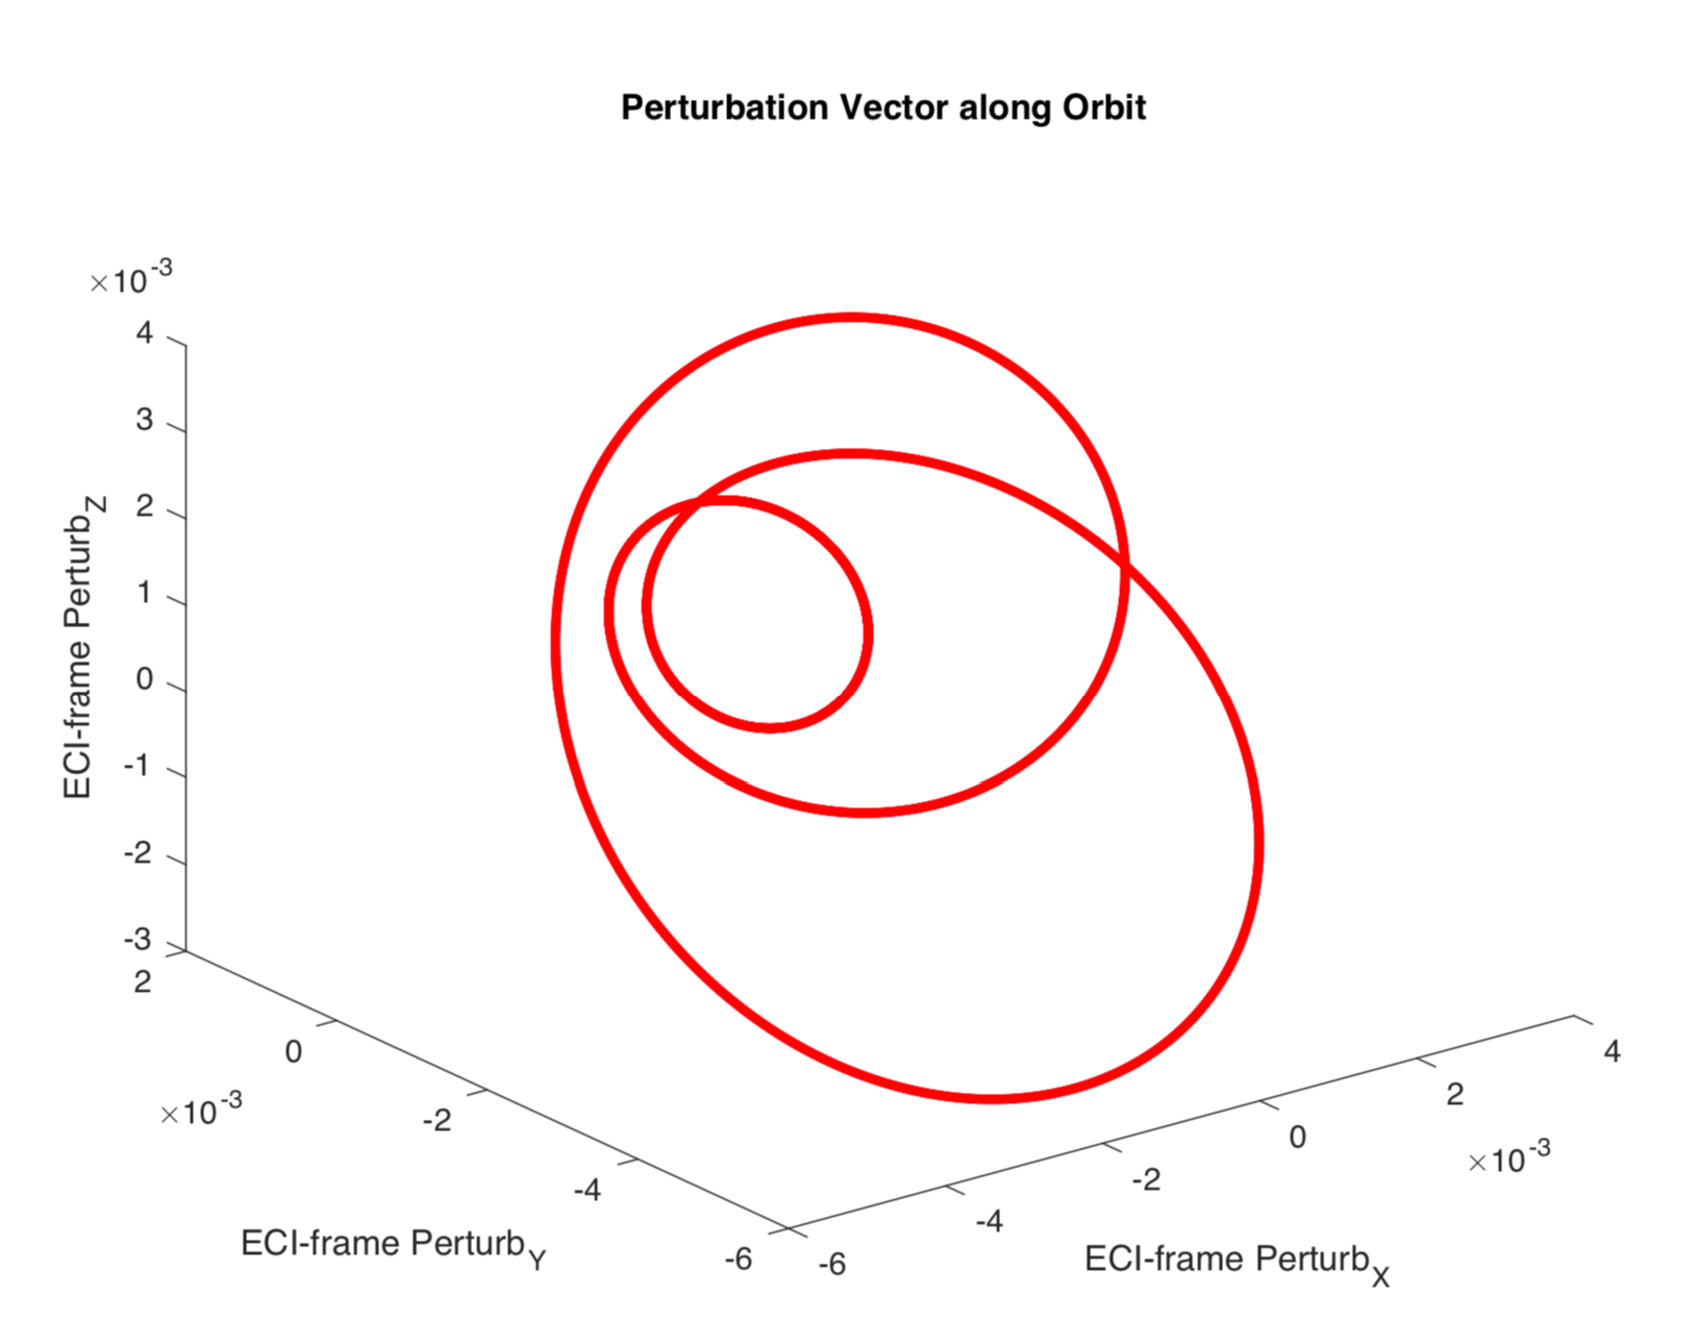
\includegraphics{EigenvaluesJ6.pdf}}
   \caption{J6 Perturbations vector transported around one orbit}
   \label{fig:J6Perturbations} 
\end{center}
\end{figure}

Given that we consider the differences between the components of the chief and the deputy to be small, the relative displacements in position and velocity space and in Kepler space should transform the way vectors transform under
change of coordinates:$$\overline{A}^j = \sum_{k=1}^m{\partial \overline{x}^j\over \partial x^k}A^k$$%with summation over the repeated index $k$ assumed by convention. 
Therefore we should be able to use a Jacobian, $\bf J$ to transform $\Delta{\bf Y} = [\hbox{$\Delta\vec{r}$}, \hbox{$\Delta\vec{v}$} ]$ displacement vectors into to Kepler space displacement vectors as follows
$$\Delta {\bf K} = {\bf J}\Delta {\bf Y} \hbox{  and the inverse relationship  } \Delta {\bf Y} = {\bf J}^{-1} \Delta {\bf K}$$Therefore the transformed equations of motion in Kepler space obtained by first going through position and velocity space looks like
$$ {\bf \dot K} = {\bf J} {\bf \dot Y} \approx {\bf J}{\bf I} + {\bf J Q J}^{-1}{\bf K}$$The transformed Homogeneous term in $K$ space is related by a similarity transformation to $\bf Q$. As long as the Jacobian $\bf J$ is invertible,the eigenvalues of $\bf Q$ and ${\bf JQJ}^{-1}$ are identical.\\

We will test out the above approach to perturbation theory and see how it compares to the canonical approach based on Lagrange's Planetary Equations. 

